\PUNT{
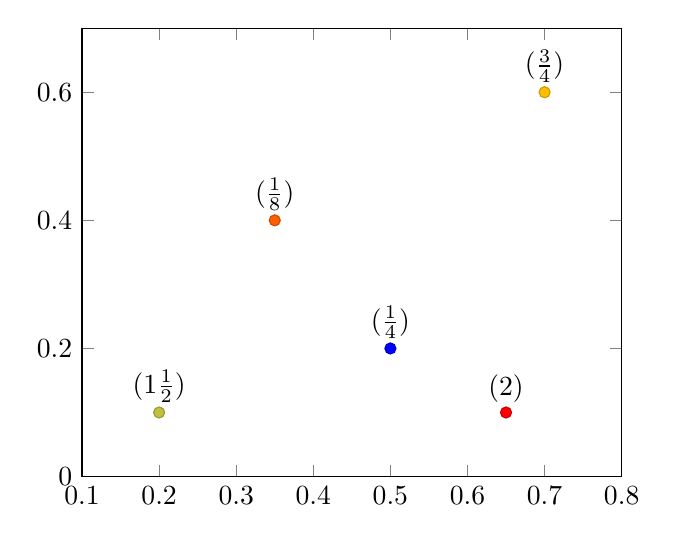
\begin{tikzpicture}
    \begin{axis}[enlargelimits=0.2]
        \addplot[
          scatter,mark=*,only marks,
          % we use 'point meta' as color data...
          point meta=\thisrow{color},
          % ... therefore, we can't use it as argument for nodes near coords ...
          nodes near coords*={$(\pgfmathprintnumber[frac]\myvalue)$},
          % ... which requires to define a visualization dependency:
          visualization depends on={\thisrow{myvalue} \as \myvalue},
        ] 
        table {
            x      y    color   myvalue
            0.5    0.2  1       0.25   
            0.2    0.1  2       1.5    
            0.7    0.6  3       0.75   
            0.35   0.4  4       0.125  
            0.65   0.1  5       2      
        };
    \end{axis}
\end{tikzpicture}


\begin{tikzpicture}
\begin{axis}[
scatter/classes={
    on={mark=square*, on},%
    off={mark=triangle*, off},%
    leo={mark=o,draw=leo}}]

    % \addplot[] is better than \addplot+[] here:
    % it avoids scalings of the cycle list
    \addplot[scatter,only marks,
        scatter src=explicit symbolic]
        coordinates {
            (0.1,0.15)  [on]
            (0.45,0.27) [leo]
            (0.02,0.17) [on]
            (0.06,0.1)  [on]
            (0.9,0.5)   [off]
            (0.5,0.3)   [leo]
            (0.85,0.52) [off]
            (0.12,0.05) [on]
            (0.73,0.45) [off]
            (0.53,0.25) [leo]
            (0.76,0.5)  [off]
            (0.55,0.32) [leo]
        };
\end{axis}
\end{tikzpicture}

}

\begin{tikzpicture}
    \begin{axis}
        [scatter/classes={
            a={mark=square*,blue},%
            b={mark=triangle*,red},%
            c={mark=o,draw=black,fill=black}%
        }]
    \addplot[
        scatter,only marks,
        scatter src=explicit symbolic]
        table[x=x,y=y,meta=label]
            {tmp/scattercl.dat};

    \addplot coordinates 
        {(0.1,0.1) (0.5,0.3) (0.85,0.5)};
    \legend{Class 1,Class 2,Class 3,Line}
\end{axis}
\end{tikzpicture}












